\documentclass{article}
\usepackage[utf8]{inputenc}
\usepackage[T1]{fontenc}
\usepackage{geometry}
\usepackage{enumitem}
\usepackage{graphicx}

\geometry{margin=0.5in}

\begin{document}
\section*{Task}
\begin{enumerate}[label=\Alph*.]
    \item Write a procedure for a moving average filter with a fixed window width and evaluate the filter's correctness. \\
    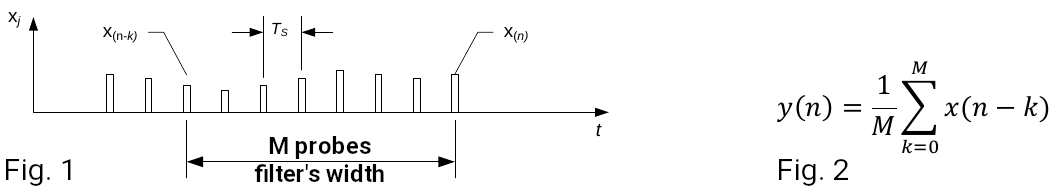
\includegraphics[width=0.95\textwidth]{../img/filter_mean_a.png} \\
    The filter averages all the signal samples within the measurement window (Fig. 1), giving equal weight to each sample. The width of the window is determined by a set number \textit{M} (the number of past samples along with the current sample) of the signal. The output value of the filter is the average of the sample values within the moving window of fixed width (Fig. 2).

    \item Assess the correctness of the filter's operation using the scheme shown below (Fig. 3) \\
    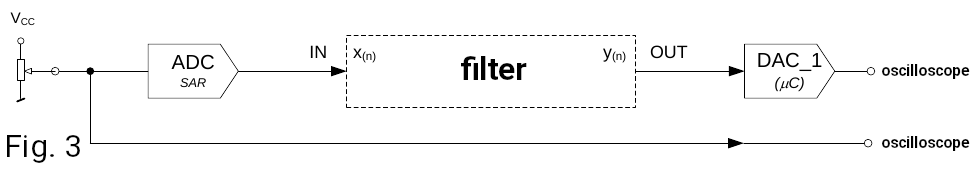
\includegraphics[width=0.95\textwidth]{../img/filter_mean_b.png}

    \item Investigate the filter's impulse and step response using the scheme shown below (Fig. 4). It requires writing a program for generating unit impulses and steps. \\
    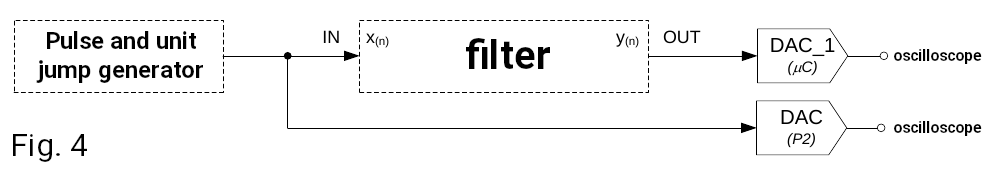
\includegraphics[width=0.95\textwidth]{../img/filter_c.png}
\end{enumerate}

\subsection*{Notes}
\begin{itemize}
    \item the samples are stored in RAM – ensure no conflict with the area occupied by the \textit{stack}
    \item suggested number of samples in the window – a power of 2
    \item for calculating the filter’s output signal, consider the possibility of exceeding the processor's word width
\end{itemize}

\subsection*{Grading}
\begin{itemize}
    \item tasks \textbf{A+B}: maximum 40 points
    \item tasks \textbf{A+B+C}: maximum 50 points
\end{itemize}

\subsection*{Suggested Literature}
R.G. Lyons, "Introduction to Digital Signal Processing," WKŁ.

\newpage
\subsection*{\textit{Appendix}}
It is possible to replace the moving average filter with a fixed window width by an FIR filter, according to one of the block diagrams shown below. \\
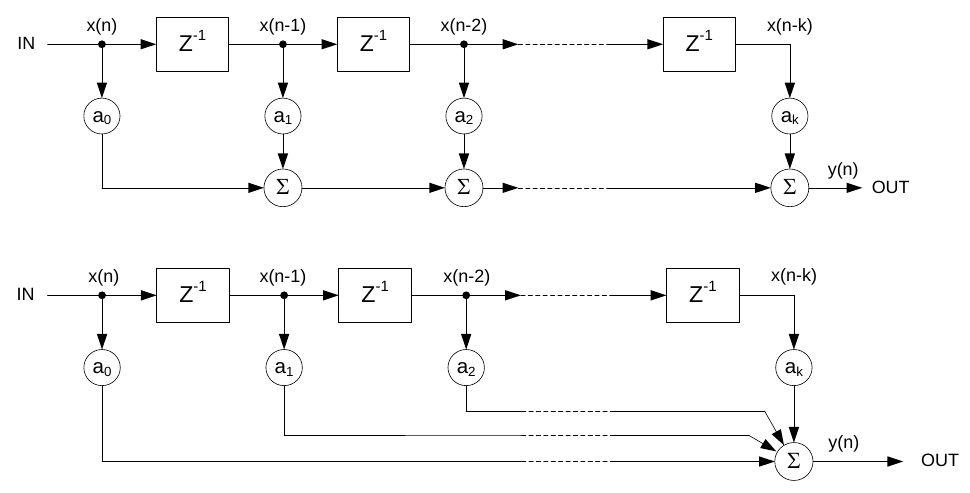
\includegraphics[width=\textwidth]{../img/filter_mean_1.png}
In that case, appropriate values for the coefficients a\textsubscript{(i)} should be chosen. This allows for proper shaping of the impulse and step responses based on the formula below, which determines the output value of the FIR filter. Therefore, it is also possible to shape the time response. \\
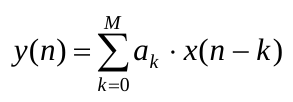
\includegraphics{../img/filter_mean_2.png}
\end{document}